\subsection{Modeling}

\begin{frame}{Modelling}{Antennas}
  \begin{columns}[T]
    \begin{column}{.5\textwidth}
      \begin{block}{}
        \begin{itemize}
          \item {Based on real directional antennas.}
          \item {Aproximated via \textit{sinc} function and assuming E and H plane symmetry.}
          \item {Focus on main lobe, HPBW (Half-power beam width) and Gain.}
        \end{itemize}
        \begin{figure}
        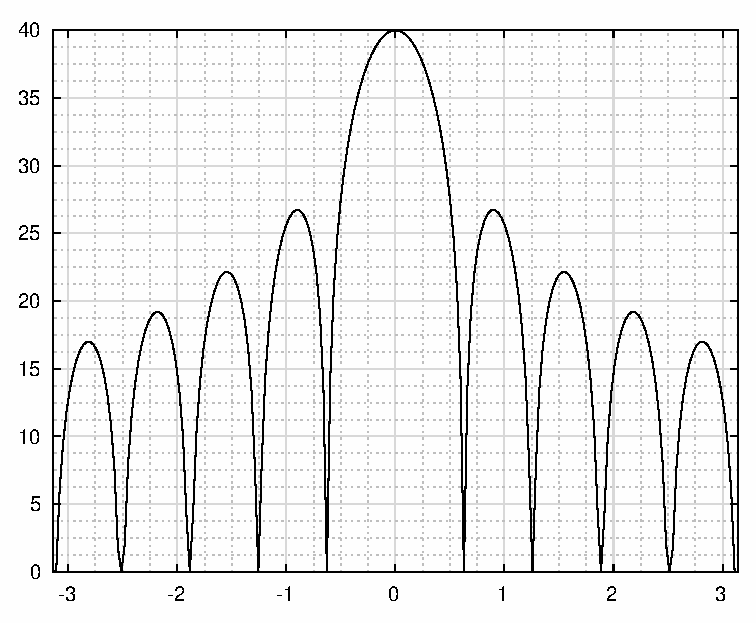
\includegraphics[scale=0.25]{figures/sinc2.eps}
      \end{figure}

      \end{block}
    \end{column}
    \begin{column}{.5\textwidth}
      \begin{figure}
        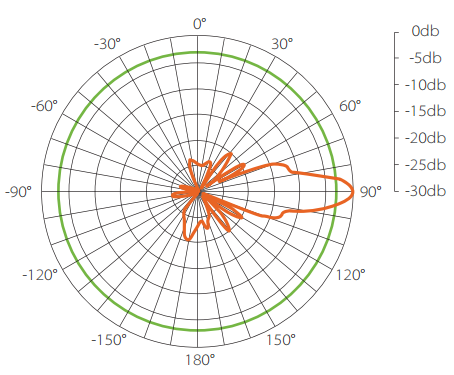
\includegraphics[scale=0.25]{figures/radpattern.png}
      \end{figure}
      \begin{figure}
        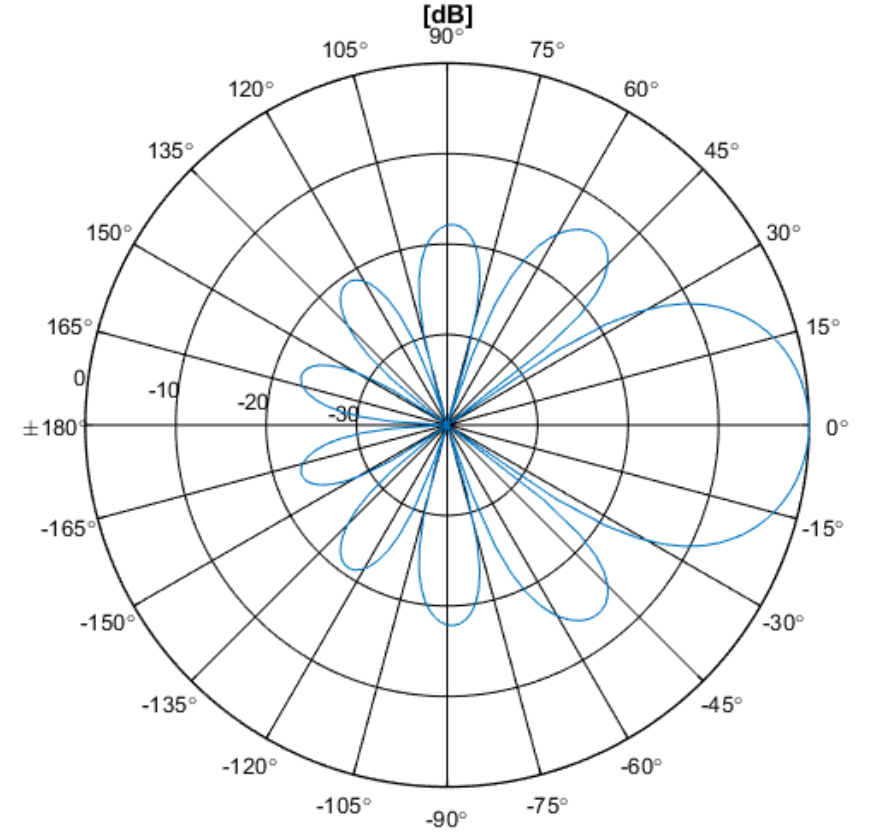
\includegraphics[scale=0.1]{figures/radpres.png}
      \end{figure}
    \end{column}
  \end{columns}
\end{frame}

\begin{frame}{Modelling}{Optimal Angles}
\begin{columns}[T]
    \begin{column}{.5\textwidth}
      \begin{block}{}
        \begin{itemize}
          \item {This calculation will be performed individually on each of the devices.}
          \item {Steps:}
          \begin{itemize}
          \item{Read GS and Drone GPS positions.}
          \item{Transform the other's device position with respect to their own NED frame.}
          \item{Perform the following calculations:}
          \end{itemize}
        \end{itemize}
      \end{block}
    \end{column}

    \begin{column}{.5\textwidth}
    \begin{figure}[H]
    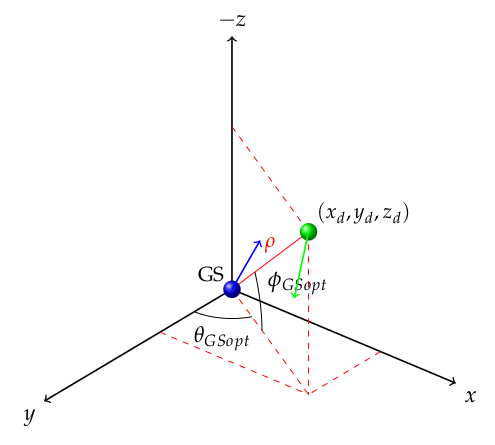
\includegraphics[scale=0.27]{figures/optimal.png}
    \end{figure}
    \end{column}
  \end{columns}
      \begin{align*}      
         \theta_{GSopt} = \text{atan2}\left(x_{d}, y_{d}\right) \nonumber \\
  \phi_{GSopt}=  \text{atan2}\left(-z_{d}, \sqrt{|x_{d}|^{2}+|y_{d}|^{2}}\right)
        \end{align*}
\end{frame}